% !TEX root = ../main.tex
% chktex-file 17
% chktex-file 21
\section{Optimizing Training}%
\label{sec:params}

Now follows an overview of approaches to speed up the training process.
We will discuss four approaches:
\begin{enumerate}
	\item A general purpose method that combines subsampling with bootstrapping.
	\item An iterative method to select the optimal subsample size during gradient descent.
	\item Improving the quality of subsampling for logistic regression by weighing the samples.
	\item Speeding up the training of SVMs via \(k\)-means clustering.
\end{enumerate}

\subsection{Bag of Little Bootstraps}%
\label{sec:params:blb}

The first approach we will discuss is called \textit{Bag of Little Bootstraps}~(BLB)~\cite{Kleiner2011}.
It is a bagging method that combines subsampling with bootstrapping and is particularly well suited for parallelized implementations.

In the context of Big Data training typically cannot be performed on the entire dataset.
A na{\"\i}ve way to solve this problem is to simply train on a random \(b\) out of \(n\) subsample of the data \(\Dtrain = \{X_1, \dots, X_n\}\).
This approach is highly sensitive to noise in the training dataset, especially if \(b \ll n\).
To overcome this problem bootstrapping can be used.
The regular \(n\) out of \(n\) bootstrapping technique for variance reduction is not suitable for big datasets because it uses \(63\%\) of the training data on average.
However the \textit{\(b\) out of \(n\) bootstrapping} (BOFN) approach can in principle be applied.
It uses \(s\) samples \(\{\check{X}^{(i)} = (\check{X}_1^{(i)}, \dots, \check{X}_b^{(i)})\, |\, 1 \leq i \leq s\}\) of \(b\) datapoints each.
Since this approach independently learns \(s\) hypotheses \(h_i\) on small datasets \(\check{X}^{(i)}\), their parameterizations \(\theta_i\) tend to have large confidence intervals.
Because of that, the quality of the combined hypothesis is strongly dependent on \(b\).
BLB reduces this dependence.

\subsubsection{Intuition}%
\label{sec:params:blb:intuition}

\begin{figure}
	\centering
	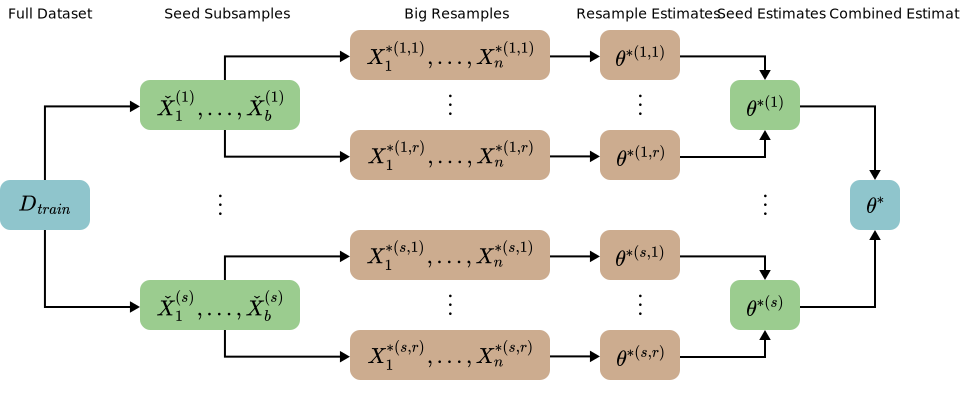
\includegraphics[width=\linewidth]{gfx/blb/overview.pdf}
	\caption{Overview of the steps of BLB.}\label{fig:blb:overview}
\end{figure}
BLB is a simple extension of BOFN that is consistently more robust regarding the choice \(b\) across datasets.
The basic idea is to add another sampling step.
BLB uses each subsample \(\check{X}^{(i)}\) as a seed for \(n\) out of \(b\) sampling.
This yields bigger resamples \(\{X^{*(i, k)} = (X_1^{*(i, k)}, \dots, X_n^{*(i, k)})\, |\, 1 \leq i \leq s, 1 \leq k \leq r\}\) that each contain at most \(b\) different elements.
Training is then run on the resamples \(X^*\) instead of the small seed samples \(\check{X}\).
The learned hypothesis parameterizations are finally combined to a single hypothesis parameterization \(\theta^*\) via a model specific combination function, e.~g.\@ by simply taking the average.
Figure~\ref{fig:blb:overview} illustrates those steps.

Even though BLB trains classifiers on resamples of size \(n\) its time and space complexity effectively still depends on \(b\), not \(n\).
This is because each resample \(X^*\) only contains at most \(b\) different elements which means that it can be efficiently represented by a list of \(b\) multiplicity counts \((c_1, \dots, c_b) \in \mathbb{N}^b\), i.~e.\@ \(\mathit{space} = \mathcal{O}(b \log n)\).
Training on such a dataset is equivalent to training on a dataset of size \(b\) with weights \(w_i = \frac{c_i}{n}\).
Since most commonly used classifiers support weighted samples, BLB is widely applicable.

\subsubsection{Evaluation}%
\label{sec:params:blb:eval}

To show the advantages of BLB for classification it was evaluated with logistic regression.
Figure~\ref{fig:blb:eval:single} shows that BLB converges on a solution much faster than the regular \(n\) out of \(n\) bootstrapping (BOOT) with comparable results.
It also shows that BLB is less sensitive to the choice of \(b\) than BOFN.\
BLB reached good results with \(b \geq n^{0.6}\) whereas BOFN required at least \(b \geq n^{0.7}\).

While BLB already outperforms BOOT without parallelism, as training is overproportionally faster on small samples, its scalability becomes more apparent when parallelized.
Figure~\ref{fig:blb:eval:parallel} shows that BLB significantly outperforms BOOT on a Spark cluster with 10 workers.
This is due to the fact that each BLB sample can be held in memory by its corresponding worker node.
The much larger BOOT samples, on the other hand, require disk reads for large datasets.
\begin{figure}
	\begin{subfigure}[t]{0.66\textwidth}
		\centering
		\includegraphics[width=0.49\linewidth]{gfx/blb/time1.pdf}
		\includegraphics[width=0.49\linewidth]{gfx/blb/time2.pdf}
		\caption{
			Single-threaded results on a subset of the data.
			\(b = n^\gamma\) for multiple values of \(\gamma \in [0.5, 1]\) and \(r = 100\) is used.
			\(s\) is not fixed and grows over time.
		}\label{fig:blb:eval:single}
	\end{subfigure}
	\hfill\
	\begin{subfigure}[t]{0.32\textwidth}
		\centering
		\includegraphics[width=\linewidth]{gfx/blb/parallel.pdf}
		\caption{
			Parallelized results on the entire dataset.
			\(b = n^{0.7}\), \(s = 5\) and \(r = 50\) is used for BLB.\
			For BOOT \(s\) grows over time.
		}\label{fig:blb:eval:parallel}
	\end{subfigure}
	\caption{
		Comparison of BLB and BOFN with BOOT using logistic regression.
		Shows the error on the moving average of all sample hypotheses that are computed within a given time.
	}\label{fig:blb:eval}
\end{figure}

\subsection{Subsample Size Selection for Gradient Descent}%
\label{sec:params:samplesize}

Next we will discuss an optimization technique for \textit{stochastic gradient descent} (SGD).
The size of the subsample \(\mathcal{S}\) that is considered in a single gradient descent step heavily influences the optimizer's behavior:
\begin{itemize}
	\item In the stochastic approximation regime small samples, typically \(|\mathcal{S}| = 1\), are used. This causes fast but noisy steps.
	\item In the batch regime large samples are used, typically \(|\mathcal{S}| = N\) with \(N := |\Dtrain|\). Steps are expensive to compute but more reliable.
\end{itemize}
Both extremes are usually not suitable for Big Data applications.
Very small samples cannot be parallelized well, making them a bad fit for the compute clusters that are typically available nowadays.
The gradients for very big samples however are often too slow to compute.
\(|\mathcal{S}|\) should ideally lie somewhere in between.

\subsubsection{Size Selection Method}%
\label{sec:params:samplesize:method}

\citet{Byrd2012} describe an iterative algorithm that dynamically increases the size of \(\mathcal{S}\) as long as this promises to significantly reduce the gradient noise.
Let \(\mathcal{S} \subseteq \{1, \dots, N\}\) describe a random subsample of \(\Dtrain = \{(x_i, y_i)\, |\, 1 \leq i \leq N\}\).
SGD will take a step in the descent direction \(d = -\nabla J_{\mathcal{S}}(w)\) where \(J_{\mathcal{S}}(w) := \frac{1}{|\mathcal{S}|} \sum_{i \in \mathcal{S}} \ell(h_{w}(x_i), y_i)\) is the differentiable average loss on \(\mathcal{S}\) given the current configuration \(w\).
Let \(J(w)\) be the average loss on the entire dataset \(\Dtrain\).
\(J(w)\) is the objective function we want to minimize.
Our goal is to trade off \(|\mathcal{S}|\) s.~t.\@ it is as small as possible and \(\nabla J_{\mathcal{S}}(w)\) still \textit{tends to agree} with the objective gradient \(\nabla J(w)\), or more formally
\begin{align}
	\|\nabla J_{\mathcal{S}}(w) - \nabla J(w) \|_2 \leq \theta \|\nabla J_{\mathcal{S}}(w)\|_2, \theta \in [0, 1)\label{eq:samplesize:cond} % chktex 9
\end{align}
A value of \(\theta = 0\) means that \(\nabla J_{\mathcal{S}}(w)\) always has to be equal to \(\nabla J(w)\),
whereas \(\theta = 1\) would allow steps that directy oppose \(\nabla J(w)\).
Since it is infeasible to compute \(\nabla J(w)\), condition (\ref{eq:samplesize:cond}) can however not be checked directly.
We will instead resort to an estimate and check whether the condition is satisfied in expectation:
\begin{align}
	\underbrace{\mathbb{E}_{\mathcal{S}}[\|\nabla J_{\mathcal{S}}(w) - \nabla J(w) \|_2^2]}_{= \|\mathrm{Var}_{\mathcal{S}}(\nabla J_{\mathcal{S}}(w))\|_1} \leq \theta^2 \|\nabla J_{\mathcal{S}}(w)\|_2^2\label{eq:samplesize:exp}
\end{align}
Computing \(\mathrm{Var}_{\mathcal{S}}(\nabla J_{\mathcal{S}}(w))\) directly is also infeasible because it would require considering all samples of a certain size.
Given a sample \(\mathcal{S}\), the variance of all samples of that size can instead be approximated by
\begin{align}
	\|\mathrm{Var}_{\mathcal{S}}(\nabla J_{\mathcal{S}}(w))\|_1 \approx \frac{1}{|\mathcal{S}| (|\mathcal{S}| - 1)} \sum_{i \in \mathcal{S}} \|\nabla \ell(h_w(x_i), y_i) - \nabla J_{\mathcal{S}}(w)\|_2^2\label{eq:samplesize:approx}
\end{align}
This approximation assumes that \(|\mathcal{S}| \ll N\).
Using (\ref{eq:samplesize:approx}) we can now estimate (\ref{eq:samplesize:exp}) which in turn estimates (\ref{eq:samplesize:cond}).
If we estimate that (\ref{eq:samplesize:exp}) is not satisfied, i.~e.\@ that the sample gradient is likely to deviate significantly from the objective gradient, a larger sample \(\widehat{\mathcal{S}}\) has to be used.
In principle we could simply increase the sample size by a constant amount repeatedly and recheck (\ref{eq:samplesize:exp}) but this is slow if \(|\mathcal{S}|\) is far off from satisfying the condition.
Instead we will adaptively choose \(|\widehat{\mathcal{S}}|\) s.~t.\@ it is expected to satisfy (\ref{eq:samplesize:exp}):
\begin{align}
	|\widehat{\mathcal{S}}| = \frac{|\mathcal{S}|\, \|\mathrm{Var}_{\mathcal{S}}(\nabla J_{\mathcal{S}}(w))\|_1}{\theta^2 \|\nabla J_{\mathcal{S}(w)}\|_2^2}\label{eq:samplesize:inc}
\end{align}
Please refer to \citet[chapter~3]{Byrd2012} for a more detailed explanation of (\ref{eq:samplesize:approx}) and (\ref{eq:samplesize:inc}).
To incorporate the ideas described above into SGD (\ref{eq:samplesize:exp}) has to be checked after each gradient descent step.
If the check fails, the size of the following samples has to be increased according to (\ref{eq:samplesize:inc}).
Good values for the initial sample size and for \(\theta\) have to be found via hyperparameter optimization.

The idea outlined above can similarly also be applied to other gradient based optimization methods like the curvature-aware \textit{Newton Conjugate Gradient} (NCG) method.
It not only uses \(\nabla J_{\mathcal{S}}(w)\) but also information from the Hessian \(\nabla^2 J_{\mathcal{S}}(w)\) to compute the direction \(d\) of the next step.
We refer to \citet[chapter~5]{Byrd2012} for the details.

\subsubsection{Evaluation}%
\label{sec:params:samplesize:eval}

Subsample size selection was evaluated on a multi-class logistic regression problem using NCG for optimization.
At first we look at the accuracy of the estimation of (\ref{eq:samplesize:cond}) via (\ref{eq:samplesize:approx}) and (\ref{eq:samplesize:exp}).
On average \(\|\mathrm{Var}_{\mathcal{S}}(\nabla J_{\mathcal{S}}(w))\|_1\) deviates about 4\% from \(\|\nabla J_{\mathcal{S}}(w) - \nabla J(w) \|_2\) on the evaluation dataset if \(|\mathcal{S}| \ll N\).

Figure~\ref{fig:samplesize:eval} shows that this accuracy is sufficient.
Dynamic subsample size selection reaches the same quality as the batch method (fixed \(|\mathcal{S}| = N\)) while using significantly fewer datapoints.
This in turn makes it significantly faster.
The speed of convergence however does depend on the choice of \(\theta\).
If \(\theta\) is too small (see \(\theta = 0.1\)), \(|\mathcal{S}|\) is increased quickly which slows down the optimization.
If \(\theta\) is too big (see \(\theta = 0.75\)), \(\nabla J_{\mathcal{S}}(w)\) is allowed to deviate significantly from \(\nabla J(w)\) which causes more erratic gradient steps.
\begin{figure}
	\begin{subfigure}{0.5\textwidth}
		\begin{tikzpicture}
			\begin{axis}[
				width=\linewidth,
				height=0.8\linewidth,
				xmin=0, xmax=6,
				ymin=0.03, ymax=0.14,
				xtick distance=1,
				ytick distance=0.02,
				xlabel={Total Number of Accessed Datapoints \(\times 10^6\)},
				ylabel={Likelihood of \(\Dtrain\)},
				axis x line=bottom,
				axis y line=left,
				label style={font=\tiny},
				tick label style={font=\tiny},
				y tick label style={/pgf/number format/.cd, fixed},
				legend style={
					at={(0.95,0.05)},
					anchor=south east,
					nodes={scale=0.6, transform shape}
				},
				legend cell align={left}
			]
				\addplot table [x=x, y=FG5, col sep=comma] {data/samplesize/performance.csv};
				\addplot table [x=x, y=FG100, col sep=comma] {data/samplesize/performance.csv};
				\addplot table [x=x, y=Dynamic, col sep=comma] {data/samplesize/performance.csv};
				\legend{Fixed \(|\mathcal{S}| = 0.05 N\),Fixed \(|\mathcal{S}| = N\),{Dynamic \(|\mathcal{S}|\), \(\theta = 0.5\)}}
			\end{axis}
		\end{tikzpicture}
	\end{subfigure}
	\begin{subfigure}{0.5\textwidth}
		\begin{tikzpicture}
			\begin{axis}[
				width=\linewidth,
				height=0.8\linewidth,
				xmin=0, xmax=6,
				ymin=0.03, ymax=0.14,
				xtick distance=1,
				ytick distance=0.02,
				xlabel={Total Number of Accessed Datapoints \(\times 10^6\)},
				ylabel={Likelihood of \(\Dtrain\)},
				axis x line=bottom,
				axis y line=left,
				label style={font=\tiny},
				tick label style={font=\tiny},
				y tick label style={/pgf/number format/.cd, fixed},
				legend style={
					at={(0.95,0.05)},
					anchor=south east,
					nodes={scale=0.6, transform shape}
				},
				legend cell align={left}
			]
				\addplot table [x=x, y=10, col sep=comma] {data/samplesize/theta.csv};
				\addplot table [x=x, y=25, col sep=comma] {data/samplesize/theta.csv};
				\addplot table [x=x, y=50, col sep=comma] {data/samplesize/theta.csv};
				\addplot table [x=x, y=75, col sep=comma] {data/samplesize/theta.csv};
				\legend{\(\theta = 0.1\), \(\theta = 0.25\), \(\theta = 0.5\), \(\theta = 0.75\)}
			\end{axis}
		\end{tikzpicture}
	\end{subfigure}
	\caption{
		Results on a multi-class logistic regression task using NCG.\
		(Left) Comparison of dynamic subsample size selection with fixed sample sizes.
		(Right) Comparison of different values for \(\theta\).
	}\label{fig:samplesize:eval}
\end{figure}

\subsection{Subsampling for Logistic Regression}%
\label{sec:params:osmac}

Subsampling usually increases the \textit{mean squared error} (MSE) of the resulting hypothesis compared to one that is trained on the full dataset \(\Dtrain\).
Let \(\mathcal{S} := \{{(x^*_i, y^*_i)\}}_{i=1}^{r}\) be a random subsample of \(\Dtrain\) that is drawn with or without replacement according to the probabilities \({\{\pi_i\}}_{i=1}^{N}\) where \(N = |\Dtrain|\) and \(\sum_{i=1}^{N} \pi_i = 1\).
Usually \(\mathcal{S}\) is drawn from a uniform distribution, i.~e.\@ each datapoint \(x_i\) is drawn with probability \(\pi_i = N^{-1}\).
Then a \textit{maximum likelihood estimate} (MLE) \(\beta_{\mathcal{S}} = (\beta_{\mathcal{S}}^{(1)}, \dots, \beta_{\mathcal{S}}^{(d)})\) is calculated as an estimate of the objective parameter vector \(\beta_{\Dtrain}\) that maximizes the likelihood of the entire dataset.
This strategy is often not optimal since some data\-points might have a smaller influence on \(\beta_{\Dtrain}\) than others.
The core idea now is to choose the probabilities \(\pi_i\) s.~t.\@ more informative datapoints are more likely to be sampled.

\subsubsection{Case Control}%
\label{sec:params:osmac:cc}

A simple idea to adjust the probabilities is to use \textit{Case-Control subsampling} (CC) in which a roughly equal amount of positive and negative samples is drawn.
Let \(\Dtrain^+ := \{(x, y) \in \Dtrain\, |\, y = 1\}\) and \(\Dtrain^- := \{(x, y) \in \Dtrain\, |\, y = 0\}\).
CC samples would be chosen without replacement with probabilities
\begin{align}
	\pi_i = \begin{cases}
		|\Dtrain^+|^{-1} & \mathrm{if}\ y_i = 1 \\
		|\Dtrain^-|^{-1} & \mathrm{if}\ y_i = 0
	\end{cases}
\end{align}
This approach however is problematic because it introduces a bias towards unambiguous samples (see fig.~\ref{fig:osmac:cc}).
\begin{figure}
	\centering
	\includegraphics[width=0.7\textwidth]{gfx/osmac/cc.png}
	\caption{Illustration of the bias introduced by CC.}\label{fig:osmac:cc}
\end{figure}

\subsubsection{Local Case Control}%
\label{sec:params:osmac:lcc}

\citet{Fithian2013} proposed \textit{Local Case-Control subsampling} (LCC) to remove the bias from CC.\
LCC determines the sampling probabilities \(\pi_i\) via a pilot estimate \(\beta_0\).
The estimate \(\beta_0\) is the MLE of a small pilot sample \(\mathcal{S}_0\) that is drawn with uniform sample probabilities.
Datapoints are now weighted by the error of the pilot estimator on them:
\begin{align}
	\pi_i = \frac{|y_i - p(x_i\, |\, \beta_0)|}{\sum_{j=1}^{N} |y_j - p(x_j\, |\, \beta_0)|}\
	\mathrm{with}\ p(x\, |\, \beta) = \frac{1}{1 + \exp(\beta^T x)}
\end{align}
Then a sample \(\mathcal{S}_{\mathrm{LCC}}\) is drawn using those probabilities, typically with replacement since this is computationally less expensive.
This produces an estimate \(\beta_{\mathcal{S}_{\mathrm{LCC}}}\) that is consistent with \(\beta_{\Dtrain}\), i.~e.\@ \(\|\beta_{\mathcal{S}_{\mathrm{LCC}}} - \beta_{\Dtrain}\|_2 \to 0\) as \(r \to \infty\).
Additionally LCC prioritizes datapoints that are close to the decision boundary estimated by the pilot.
This tends to reduce the variance of the estimate \(\beta_{\mathcal{S}_{\mathrm{LCC}}}\), especially if \(\Dtrain\) contains an imbalanced amount of positive and negative samples.

\subsubsection{OSMAC}%
\label{sec:params:osmac:idea}

While LCC tends to reduce the estimate's variance, it does not necessarily minimize it.
The \textit{\textbf{O}ptimal \textbf{S}ubsampling \textbf{M}otivated by the \textbf{A}-Optimality \textbf{C}riterion} (OSMAC)~\cite{Wang2017} method improves upon LCC by minimizing the expected variance.\
Like LCC it also uses a pilot estimate \(\beta_0\) but the sampling probabilities \(\pi_i\) are then calculated differently.

Let \(V := \mathrm{Cov}(\beta_{\mathcal{S}} - \beta_{\Dtrain})\) be the covariance matrix of the difference between the sample estimate and the complete dataset estimate.
Given \(\mathbb{E}[\beta_{\mathcal{S}} - \beta_{\Dtrain}] = \mathbf{0}\), \(V\) can be interpreted as a measure of the expected error introduced by subsampling.
Using the A-optimality criterion of optimal design, OSMAC sets the sampling probabilities \(\pi_i\) so that \(\mathrm{tr}(V)\) is minimized in expectation.
More intuitively this minimizes the sum of the MSEs on the regression coefficients \(\beta_{\mathcal{S}}^{(k)}\), i.~e.\@ \(\sum_{k=1}^{d} \mathbb{E}[(\beta_{\mathcal{S}}^{(k)} - \beta_{\Dtrain}^{(k)})^2]\). % chktex 3

It turns out that finding the minimizing probabilities \(\pi_i\) of \(\mathrm{tr}(V)\) is computationally expensive.
However the optimal values for \(\pi_i\) can be approximated using
\begin{align}
	\pi_i = \frac{|y_i - p(x_i\, |\, \beta_0)| \cdot \|x_i\|_2}{\sum_{j=1}^{N} |y_j - p(x_j\, |\, \beta_0)| \cdot \|x_j\|_2}\label{eq:osmac:approx}
\end{align}
The only difference to LCC here is the added \(\|x_i\|_2\) factor.
The intuition behind this is that samples with large norms tend to be further away from the decision boundary%
\footnote{
	This intuition is not entirely correct since it does not consider the offset and rotation of the decision boundary.
	Those aspects are ignored because (\ref{eq:osmac:approx}) only approximates the A-optimal probabilities.
	For details please refer to \citet[chapter 3.2]{Wang2017}.
}.
An incorrectly classified sample that is far from the decision boundary is more surprising than an incorrectly classified sample close to it.
Since the sigmoidal \(p\) function saturates quickly this fact is often not captured by LCC sampling.

\subsubsection{Evaluation}%
\label{sec:params:osmac:eval}

We will now compare uniform, LCC and OSMAC sampling on the two datasets.
The datapoints \(x_i\) are randomly sampled from different distributions.
The corresponding classes \(y_i \in \{0, 1\}\) are then assigned using a fixed coefficient vector \(\beta\).
These two datasets are used:
\begin{itemize}
	\item \textbf{mzNormal:}
		Uses a multivariate normal distribution \(\mathcal{N}(0, \Sigma)\) with mean \(0\) and \(\Sigma_{i j} = 0.5^{\delta_{i \neq j}}\).
		Contains a roughly equal amount of positive and negative samples.
	\item \textbf{nzNormal:}
		Uses a multivariate normal distribution \(\mathcal{N}(1.5, \Sigma)\) with mean \(1.5\).
		About 95\% of the samples are positive.
\end{itemize}

Figure~\ref{fig:osmac:mse} shows the MSEs \(\|\beta_{\mathcal{S}} - \beta\|_2^2\) for different subsample sizes \(r\).
OSMAC consistently gives the closest approximation of \(\beta\), confirming its theoretical A-optimality.
\begin{figure}[t]
	\begin{subfigure}{0.5\textwidth}
		\begin{tikzpicture}
			\begin{axis}[
				width=\linewidth,
				height=0.8\linewidth,
				xmin=100, xmax=1000,
				ymin=0, ymax=0.8,
				xtick distance=200,
				ytick distance=0.2,
				xlabel={\(r\)},
				ylabel={MSE},
				axis x line=bottom,
				axis y line=left,
				label style={font=\tiny},
				tick label style={font=\tiny},
				y tick label style={/pgf/number format/.cd, fixed},
				legend style={
					at={(0.95,0.95)},
					anchor=north east,
					nodes={scale=0.6, transform shape}
				},
				legend cell align={left}
			]
				\addplot table [x=x, y=uniform, col sep=comma] {data/osmac/mse-mzNormal.csv};
				\addplot table [x=x, y=LCC, col sep=comma] {data/osmac/mse-mzNormal.csv};
				\addplot table [x=x, y=OSMAC, col sep=comma] {data/osmac/mse-mzNormal.csv};
				\addplot [dashed] table [x=x, y=full, col sep=comma] {data/osmac/mse-mzNormal.csv};
				\legend{uniform, LCC, OSMAC, full}
			\end{axis}
		\end{tikzpicture}
		\caption{mzNormal}
	\end{subfigure}
	\begin{subfigure}{0.5\textwidth}
		\begin{tikzpicture}
			\begin{axis}[
				width=\linewidth,
				height=0.8\linewidth,
				xmin=100, xmax=1000,
				ymin=0, ymax=2.5,
				xtick distance=200,
				ytick distance=0.5,
				xlabel={\(r\)},
				ylabel={MSE},
				axis x line=bottom,
				axis y line=left,
				label style={font=\tiny},
				tick label style={font=\tiny},
				y tick label style={/pgf/number format/.cd, fixed},
				legend style={
					at={(0.95,0.95)},
					anchor=north east,
					nodes={scale=0.6, transform shape}
				},
				legend cell align={left}
			]
				\addplot table [x=x, y=uniform, col sep=comma] {data/osmac/mse-nzNormal.csv};
				\addplot table [x=x, y=LCC, col sep=comma] {data/osmac/mse-nzNormal.csv};
				\addplot table [x=x, y=OSMAC, col sep=comma] {data/osmac/mse-nzNormal.csv};
				\addplot [dashed] table [x=x, y=full, col sep=comma] {data/osmac/mse-nzNormal.csv};
				\legend{uniform, LCC, OSMAC, full}
			\end{axis}
		\end{tikzpicture}
		\caption{nzNormal}
	\end{subfigure}
	\caption{MSEs on \(\beta\) for different subsample sizes \(r\).}\label{fig:osmac:mse}
\end{figure}

\subsection{Clustering for SVMs}%
\label{sec:params:wkmsvm}

To speed up the training of SVMs \citet{Almeida2000} proposed a simple method that reduces the dataset size via \(k\)-means clustering.
It can be described as a simple three-step procedure:
\begin{enumerate}
	\item Group the training samples \(\Dtrain\) into \(k\) clusters \(C_1, \dots, C_k\) with centers \(c_1, \dots, c_k\) where \(k\) should be determined via hyperparameter optimization.
	\item Check for each cluster \(C_i\) whether all associated datapoints belong to the same class, i.~e.\@ \(\exists\, z \in \{+1, -1\}: \forall (x, y) \in C_i: y = z\).
		If yes, all datapoints in \(C_i\) are removed from \(\Dtrain\) and replaced by \(c_i\).
		If not, they are kept in the dataset.
		The intuition behind this is that clusters with points from multiple classes might be near the decision boundary so they are kept to serve as potential support vectors.
	\item Finally standard SVM training is performed on the reduced training dataset.
\end{enumerate}
This approach performs similarly to SVM training on the full dataset.
However the size of the reduced dataset is very unpredictable.
Large homogeneous clusters with only a few noisy outliers of a different class will not be used to reduce the dataset size.
Because of that the effective speedup and memory requirements may vary greatly depending on the dataset.

\citet{Lee2007} proposed KM-SVM, an alternative approach that solves this problem by performing clustering on the datapoints of each class separately.
This method has more predictable time and memory requirements but it also tends to modify the structure of the dataset.
Figure~\ref{fig:wkmsvm:compare:km} shows that this can cause KM-SVM to deviate significantly from the full dataset SVM.\
\begin{figure}
	\begin{subfigure}{0.5\textwidth}
		\centering
		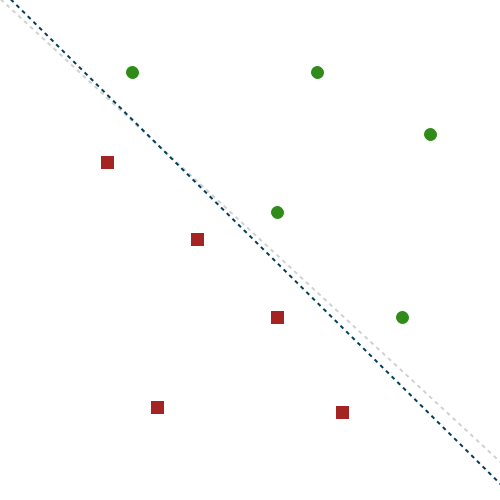
\includegraphics[width=0.85\linewidth]{gfx/wkmsvm/km.png}
		\caption{KM-SVM}\label{fig:wkmsvm:compare:km}
	\end{subfigure}
	\begin{subfigure}{0.5\textwidth}
		\centering
		\includegraphics[width=0.85\linewidth]{gfx/wkmsvm/wkm.png}
		\caption{WKM-SVM}\label{fig:wkmsvm:compare:wkm}
	\end{subfigure}
	\caption{Comparison of the decision boundaries of KM-SVM and WKM-SVM.}\label{fig:wkmsvm:compare}
\end{figure}

WKM-SVM~\cite{Bang2014} improves upon KM-SVM by weighting each cluster center \(c_i\) by the amount of datapoints \(|C_i|\) it represents.
This solves the problem that small clusters of outliers have the same influence on the decision boundary as big clusters of more representative datapoints in KM-SVM.\
Figure~\ref{fig:wkmsvm:compare:wkm} shows how this improves the quality of the decision boundary.

\subsubsection{Evaluation}%
\label{sec:params:wkmsvm:eval}

We will now compare KM-SVM and WKM-SVM using different compression rates \(R \in \{1, 3, 5, 10\}\) that describe the number of clusters \(k = \frac{|\Dtrain|}{R}\).
A compression rate of \(R = 1\) corresponds to a SVM that is trained on the entire dataset.
For \(\Dtrain\) the \texttt{PimaIndiansDiabetes2} dataset is used.
Figure~\ref{fig:wkmsvm:eval} shows that WKM-SVM consistently performs better than KM-SVM with a roughly identical training time.

\begin{figure}
	\begin{subfigure}{0.33\textwidth}
		\begin{tikzpicture}
			\begin{axis}[
				width=\linewidth,
				height=0.8\linewidth,
				xmin=1, xmax=10,
				ymin=0.2, ymax=0.3,
				xtick={1,3,5,10},
				ytick distance=0.02,
				xlabel={\(R\)},
				ylabel={Test error},
				axis x line=bottom,
				axis y line=left,
				label style={font=\tiny},
				tick label style={font=\tiny},
				y tick label style={/pgf/number format/.cd, fixed},
				legend style={
					at={(0.05,0.95)},
					anchor=north west,
					nodes={scale=0.6, transform shape}
				},
				legend cell align={left}
			]
				\addplot table [x=compression, y=km-err, col sep=comma] {data/wkmsvm/diabetes.csv};
				\addplot table [x=compression, y=wkm-err, col sep=comma] {data/wkmsvm/diabetes.csv};
				\legend{KM, WKM}
			\end{axis}
		\end{tikzpicture}
	\end{subfigure}
	\begin{subfigure}{0.33\textwidth}
		\begin{tikzpicture}
			\begin{axis}[
				width=\linewidth,
				height=0.8\linewidth,
				xmin=1, xmax=10,
				ymin=0, ymax=1250,
				xtick={1,3,5,10},
				ytick distance=200,
				xlabel={\(R\)},
				ylabel={Training time (sec)},
				axis x line=bottom,
				axis y line=left,
				label style={font=\tiny},
				tick label style={font=\tiny},
				y tick label style={/pgf/number format/.cd, fixed},
				legend style={
					at={(0.95,0.95)},
					anchor=north east,
					nodes={scale=0.6, transform shape}
				},
				legend cell align={left}
			]
				\addplot table [x=compression, y=km-time, col sep=comma] {data/wkmsvm/diabetes.csv};
				\addplot table [x=compression, y=wkm-time, col sep=comma] {data/wkmsvm/diabetes.csv};
				\legend{KM, WKM}
			\end{axis}
		\end{tikzpicture}
	\end{subfigure}
	\begin{subfigure}{0.32\textwidth}
		\begin{tikzpicture}
			\begin{axis}[
				width=\linewidth,
				height=0.8\linewidth,
				xmin=1, xmax=10,
				ymin=0, ymax=185,
				xtick={1,3,5,10},
				ytick distance=25,
				xlabel={\(R\)},
				ylabel={Support vectors},
				axis x line=bottom,
				axis y line=left,
				label style={font=\tiny},
				tick label style={font=\tiny},
				y tick label style={/pgf/number format/.cd, fixed},
				legend style={
					at={(0.95,0.95)},
					anchor=north east,
					nodes={scale=0.6, transform shape}
				},
				legend cell align={left}
			]
				\addplot table [x=compression, y=km-sv, col sep=comma] {data/wkmsvm/diabetes.csv};
				\addplot table [x=compression, y=wkm-sv, col sep=comma] {data/wkmsvm/diabetes.csv};
				\legend{KM, WKM}
			\end{axis}
		\end{tikzpicture}
	\end{subfigure}
	\caption{Comparison of KM-SVM and WKM-SVM.}\label{fig:wkmsvm:eval}
\end{figure}
